\chapter{A Játék avagy A TCGE}

\section{Alap ötlet}

A játék avagy a TCGE (The card game ever) alap ötlete az RPG és kártya játékok fúzionálása egy saját kis csavarral. A játék egy fizikai kártyajátékra épül melyet én és barátom (Hoszowski Hubert) hozotunk létre. A játék eredetileg 6 karakter klasst tartalmazott melyek a: Warrior (Harcos), Ranger (Íjjász), Mage (Mágus), Druid (Druida), Paladin (Lovag), Ninja (Nindzsa). 

Ezek bővítve lettek az Alchemist (Alkémista) illetve a Necromancer (Nekromanta) klassokkal. A játék egy TTRPG (Table Top Role Play Game) formulát követte miszerint van egy mesélő aki vezeti a történetet,a játékos pedig mesélőn kersztül tud interaktálni a környezettel. Az esetleges ellenszenves interakciók illetve csaták pedig a kártyajáték rendezte.

A mesélői szerep a project során átalakításra került mivel a project fókusza nem a történet mesélésen volt hanem a kártyajáték elkészítésén.


\section{Technológia}

A program Unity engine-ben készült, C\# nyelven. Az elkészült grafikák a Krita nevezetű rajzporgramban készültek. A unity nagyon hasznosnak bizonyult a játék készítése során mivel így nem volt szükség egy keretrendszer vagy játék motor elkészítésére.   

\clearpage
\section{Főmenü}

A játék indítását követően a főmenü fogadja a játékost. A menü interaktív. Ez azt jelenti hogy képernyő közepén lévő gombok helyett a háttér egyes elemeire kattintva tudjuk a külömböző funkciókat elérni.

\begin{figure}[h]
        \centering
        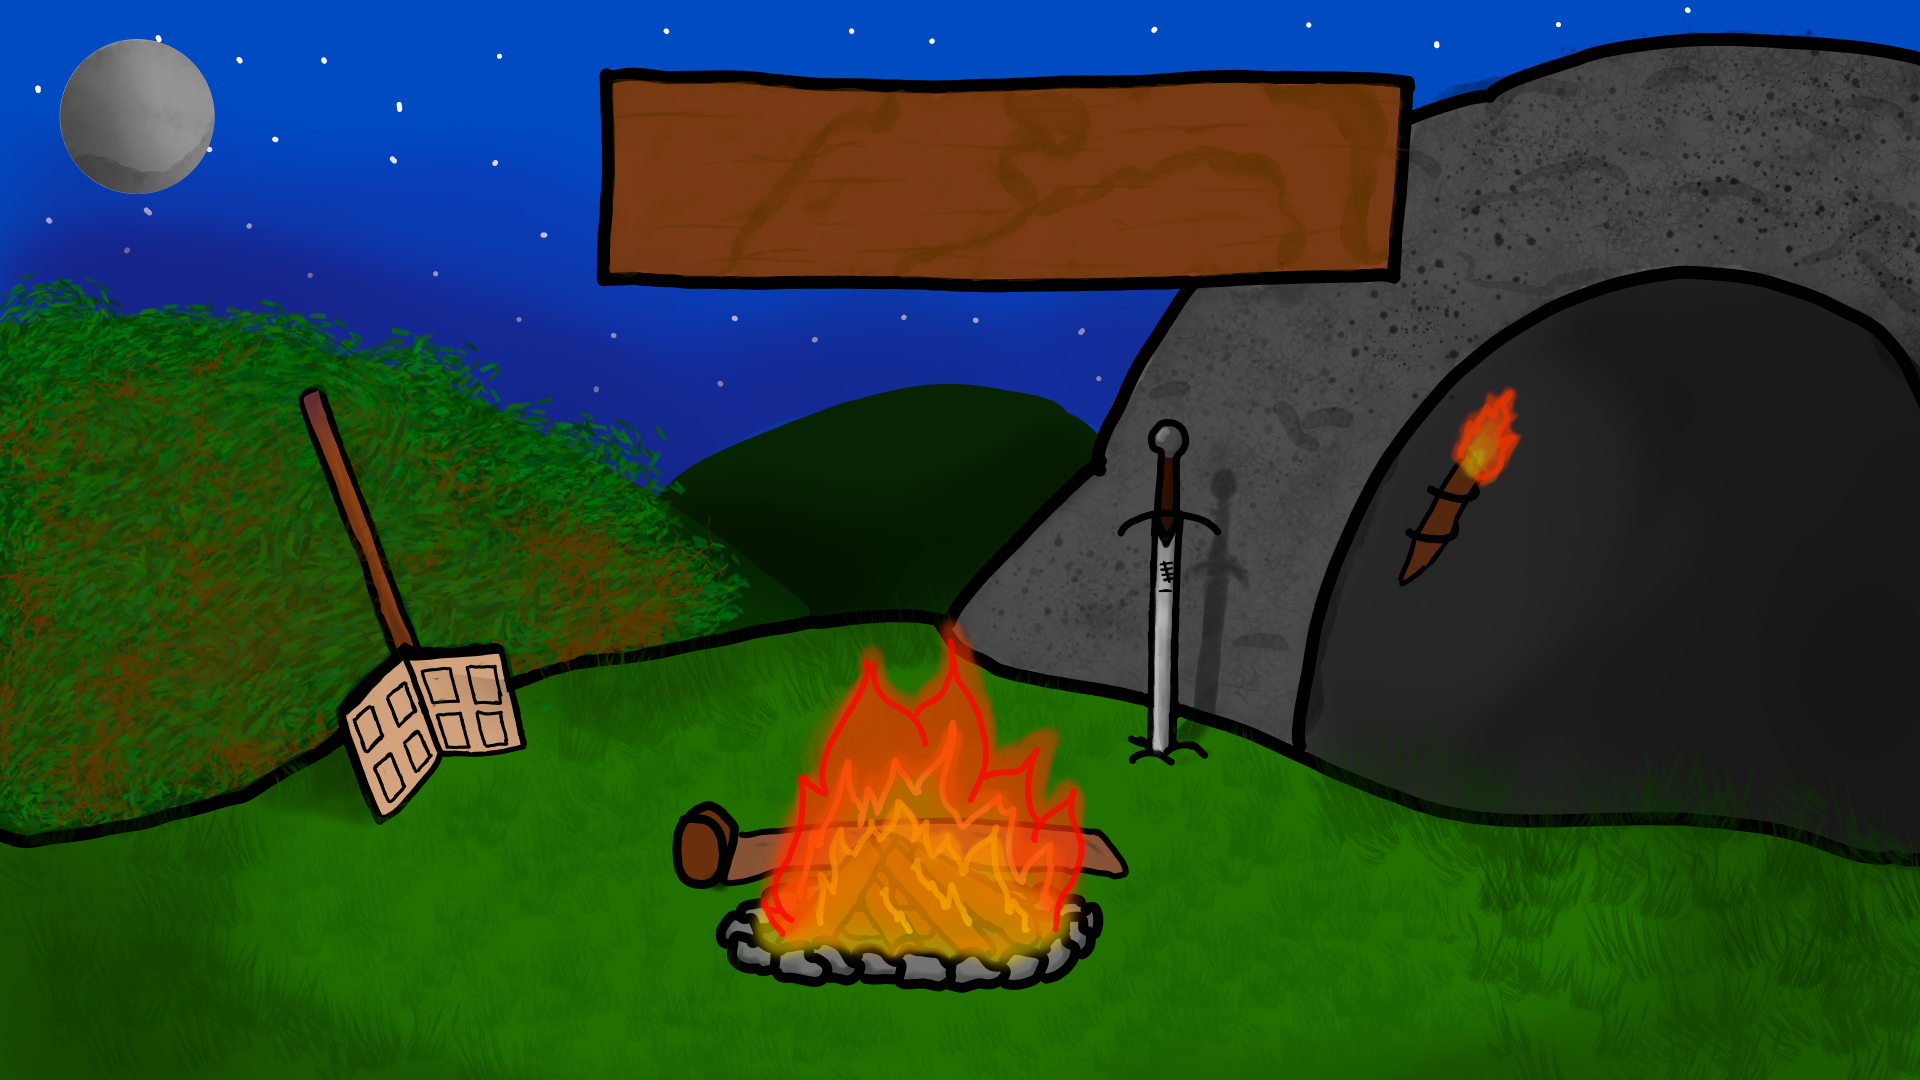
\includegraphics[width=400px,keepaspectratio]{images/Menu.png}
        \caption {A játék menüje}
        \label{Menü}
    \hspace{1em}
\end{figure}
\begin{figure}[h]
        \centering
        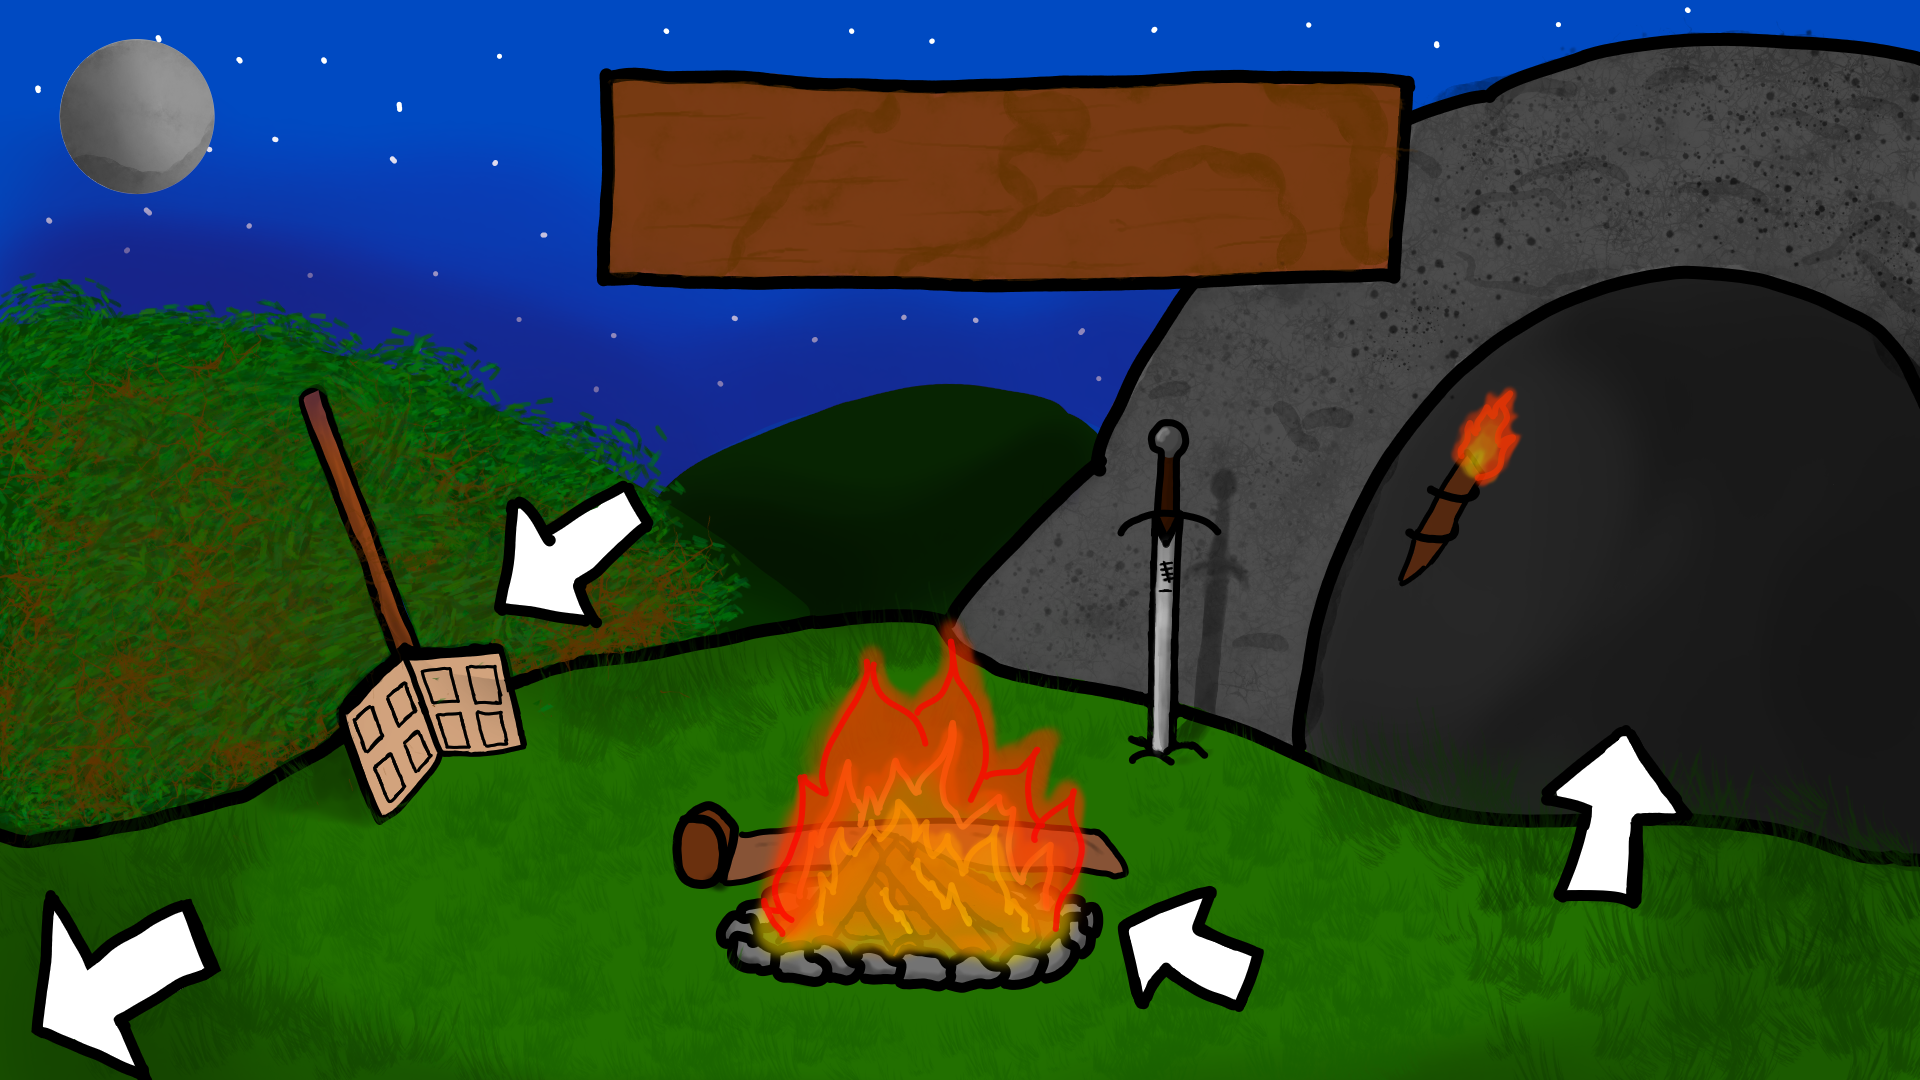
\includegraphics[width=400px,keepaspectratio]{images/menü_with_arrows.png}
        \caption {Interaktív elemek}
        \label{Menü_with_arrows}
    \hspace{1em}
\end{figure}
\clearpage
\subsection{Funkciók}
\subsubsection{Barlang}
A barlangva kattintva idítható el a játék. A játék megkezdése előtt a játékosnak egy Klass-t kell választania. A Klassz választás egy felugró felületen történik ahol mind a 8 Klass meg van jelenítve. A jobb felső sarokban található egy Close gomb amivel be lehet zárni a menüt.
\subsubsection{Tábor tűz}
A tábor tűzre kattintva a játékos a beállítások menübe kerül. Itt tudja a játékos a felbontást beállítani.
\subsubsection{Gyűjtő könyv}
A könyvre kattintva a játékos megnézheti a játékban szereplő kártyákat. Ha a kurzort a kártya felé viszi, a képernyő közepén a kártya megjelenik. A felület két oldalán található egy egy gomb ami lapozási lehetőséget ad a kártyák között. A jobb felső sarokban található a Close gomb amire kattintva a felület bezárja magát.
\subsubsection{Bal Sarok}
A bal sarokba kattintva a játékos kilép a játékból. Ezen felül az Esc gombot lenyomva kiléphetünk az aplikációbol.

\section{Karakter választó}

Miután a főmenüben elindítottuk az új játékot először választanunk kell a játékban
szereplő 8 klass kötül. Ezek mind más-más játékstílussal bírnak a játékos számára.
Miután kiválasztotta a kasztját egy kezdő paklit kap a játékos.
\begin{figure}[h]
        \centering
        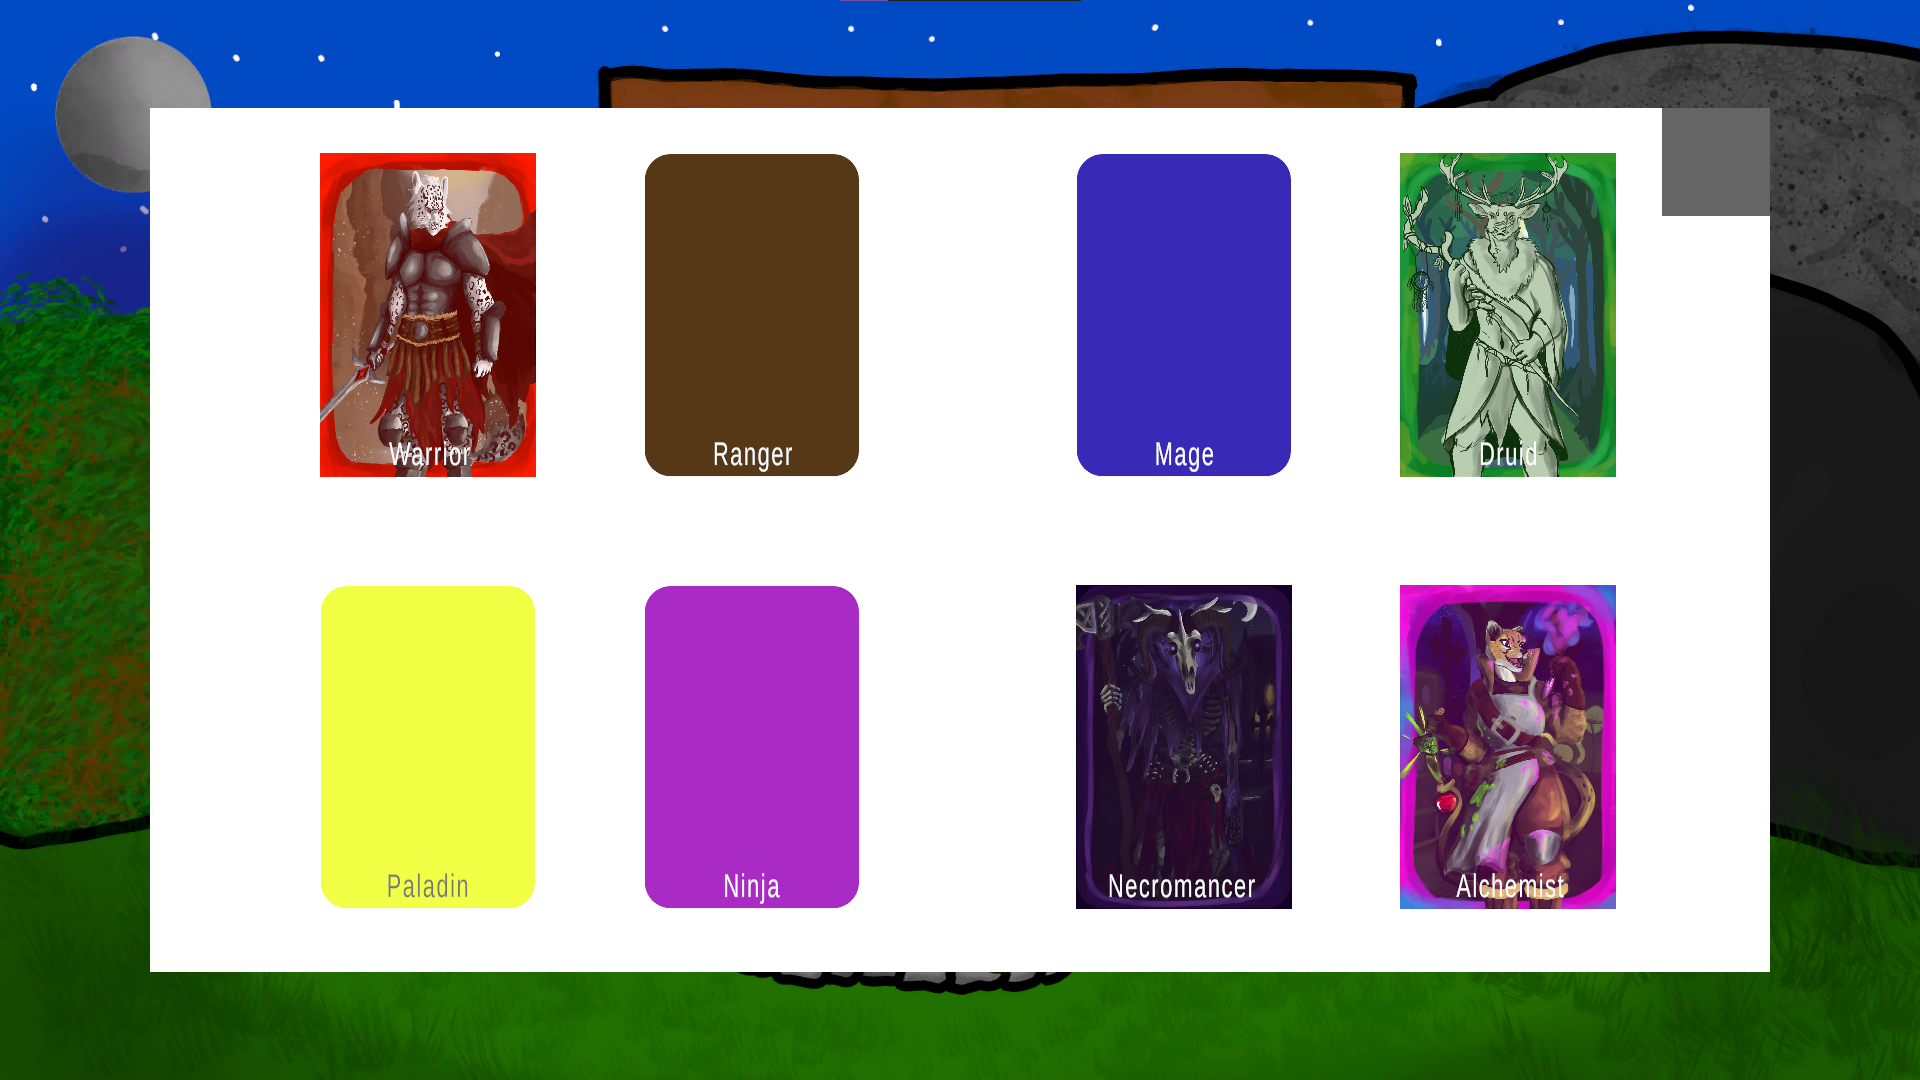
\includegraphics[width=400px,keepaspectratio]{images/CharSelect.png}
        \caption {Karakter választó}
        \label{Karakter_selektor}
    \hspace{1em}
\end{figure}
\clearpage

\section{Aréna}
Miután kiválasztottuk a karakterünket bekerülünk az arénába. Ezen a ponton kezdődik a tényleges játék része az programnak.
\begin{figure}[h]
        \centering
        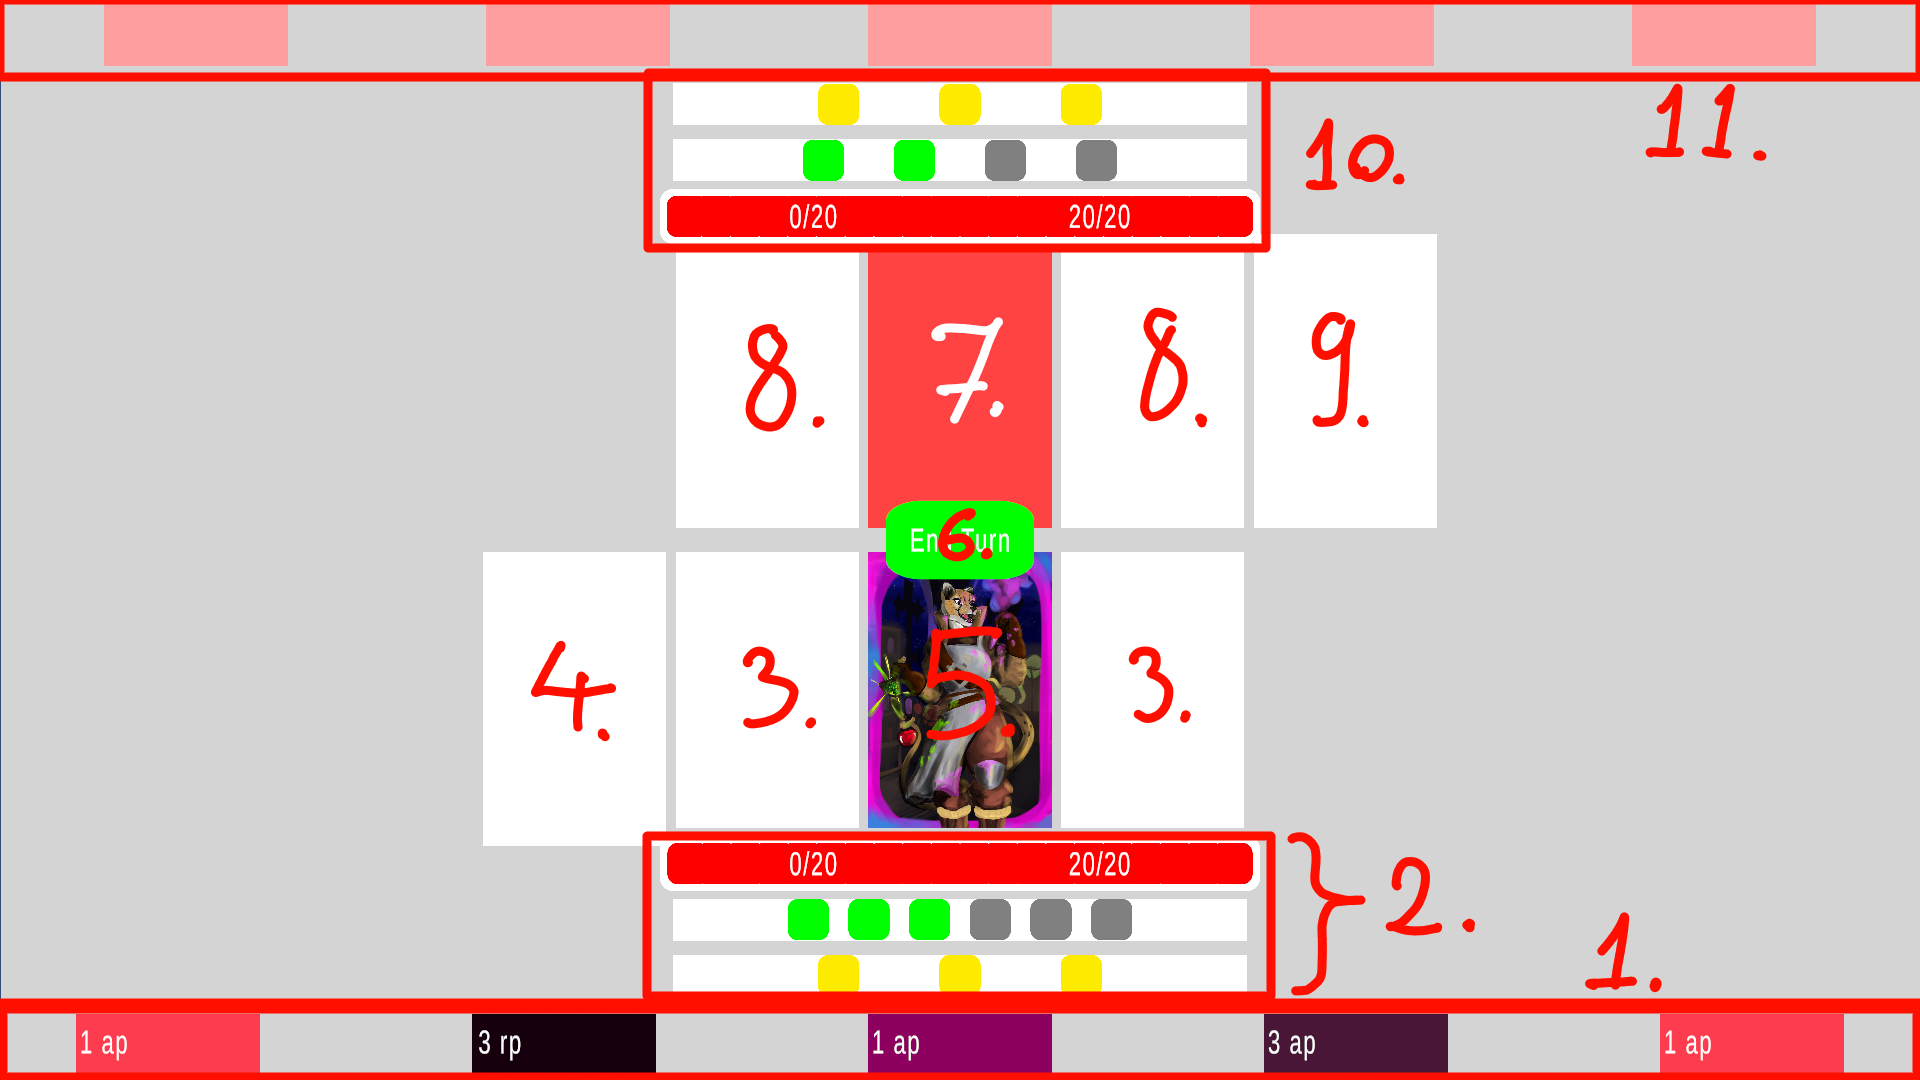
\includegraphics[width=400px,keepaspectratio]{images/BoardExpl.png}
        \caption {Az aréna}
        \label{Arena_full}
    \hspace{1em}
\end{figure}
\subsection{Játékos keze}
Ez a játékos keze. Ide kerülnek a kijátszható lapok a pakliból.
\subsection{Játékos pontjai}
A játékos 4 pontal rendelkezik. Fentről lefelé indulva ezek a:
\begin{itemize}
    \item Pajzs pontok. Ezek mutatják hogy a játékosnak mennyi pajzsa van. A pajzsok csökkentik a beérkező sebzést amit a játékos kapna. Ez a baloldali érték.
    \item Élet pontok. Ezek mutatják meg hogy a játékosnak mennyi maximum életereje illetve jelenleg mennyi életereje van még. Ha ez leesik nullára a játékos veszít. Ez a jobboldali érték.
    \item Akció pontok. Ez az erőforrás egyes kártyák kijátszására használható. Ezek egy részét a játékos visszanyeri a köre elején.
    \item Reakció pontok. Ez az erőforrás más kártyák kijátszására használható fel. a köre elején a játékos visszanyeri az összes reakció pontját.
\end{itemize}
\subsection{Felszerelés és idézett lények}
Ezekbe a kártya helyekbe Felszerelések és idézett lények tehetőek amik segítséget nyújtanak csata közben. Ezek a segítségek lehetnek: a fizikai sebzés növelése, mágikus sebzés növelése, extra sebzés az ellenfélbe, gyógyítás vagy akár extra kártya húzas. 
\subsection{Aréna effectus}
Az aréna effectusok hasnolóak a felszerelésekhez, de csak erre az egy helyre kerülhet. Az aréna effektusok speciális tulajdonságokkal rendelkeznek mint például: a játékos akciópont visszanyerésének növelése vagy pajzs adása akkor hogyha a játékos annyi sebzést szenved el hogy az túlütné a pajzsainak számát.
\subsection{Játékos karaktere}
Itt található a játékos karaktere
\subsection{Kör vége gomb}
Erre rányomva a játékos lezárhatja a körét. Ha zöld a játékos köre van éppen, ha piros akkor pedig az ellenfélé.
\subsection{Ellenfél karaktere}
Ez az ellenfélé karakterének helye.
\subsection{Ellenfél felszerelés}
Ez az ellenfélé felszerelésének helye helye.
\subsection{Ellenfél Aréna effektus}
Ez az ellenfélé aréna effektusának helye helye.
\subsection{Ellenfél pontjai}
Hasonlóan a játékoshoz az ellenfél is rendelkezik: pajzs-, élet-, akció- és reakció pontokkal melyek ugyan úgy működnek mint a játékos pontjai.
\subsection{Ellenfél Kártyáji}
Ez is hasonló a játékos kezéhez az ellenfél a köre során kijátszik kártyákat.
\clearpage

Attól függően hogy az Arénát győztesként vagy vesztesként fejeztük be úgy változik a tovább haladásunk. Ha győztünk egy felugró ablak jelzi számunkra ezt a tényt és a rajta szereplő Continue (folytatás) gombra kattintva tövább léphetünk.

\begin{figure}[h]
        \centering
        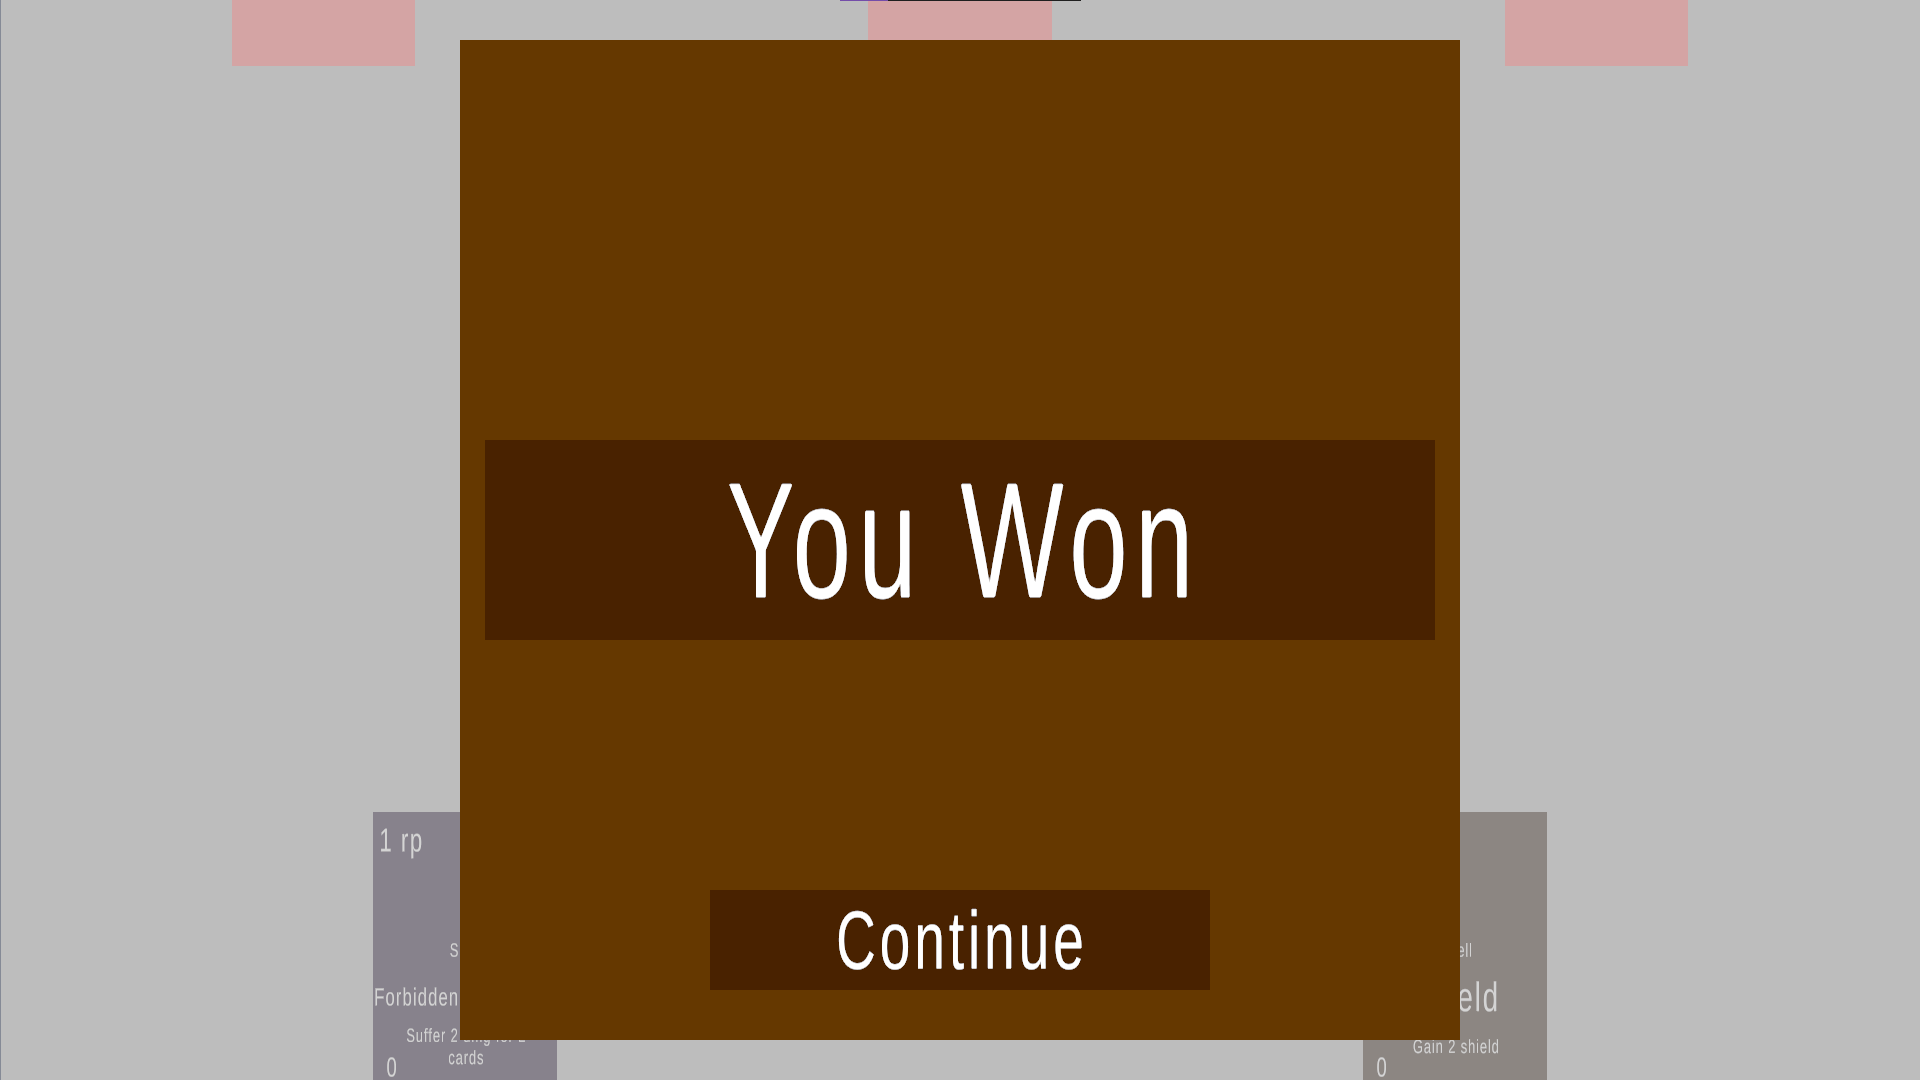
\includegraphics[width=400px,keepaspectratio]{images/won.png}
        \caption {Felugró kép győzelem esetén}
        \label{Won}
    \hspace{1em}
\end{figure}

Ha vesztettünk akkor egy hasonló ablak vár minket ami közli velünk hogy vesztettünk és egy gomb ami pedig vissza visz minket a főmenübe ahol újra kezdhetjük a kalandunkat. 

\begin{figure}[h]
        \centering
        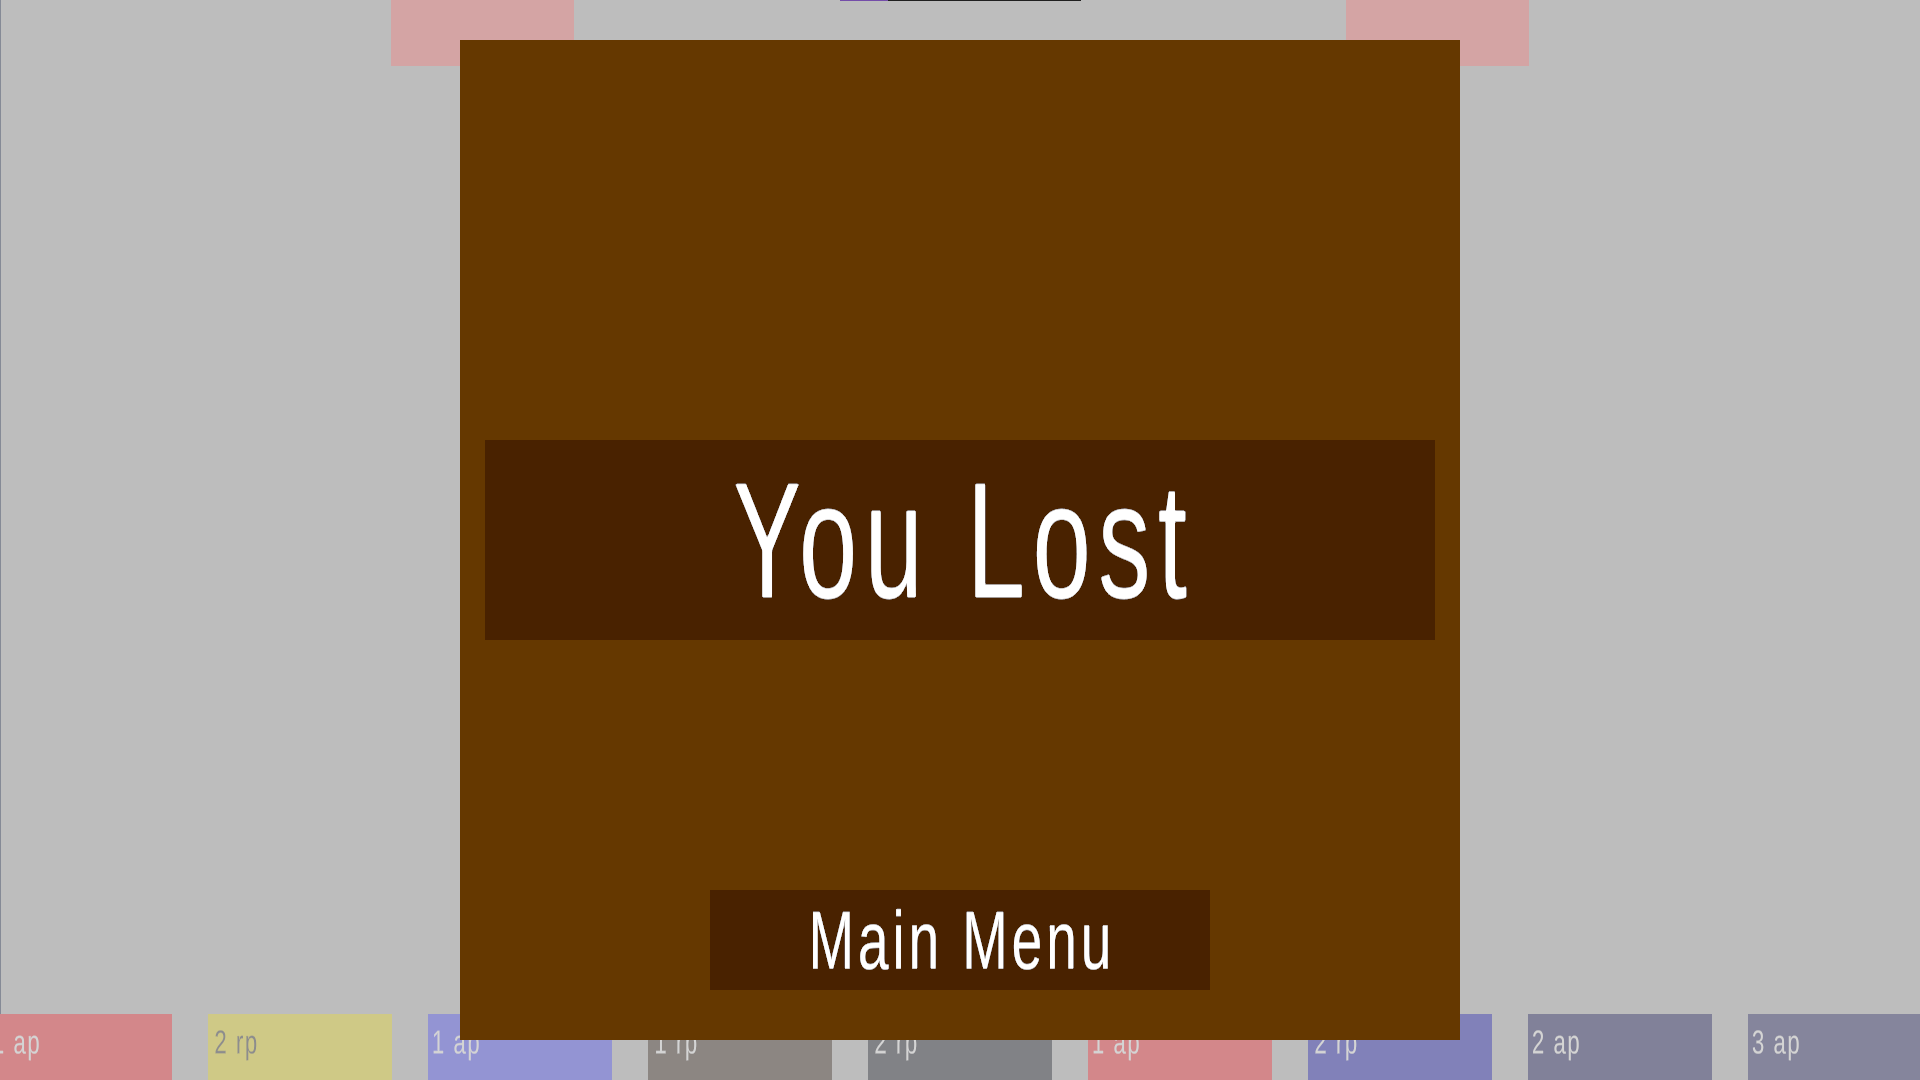
\includegraphics[width=400px,keepaspectratio]{images/lost.png}
        \caption {Felugró kép vesztés esetén}
        \label{lost}
    \hspace{1em}
\end{figure}

\clearpage
\section{Kártya Választás}

Miután nyertünk tovább kerülünk a kártya választó felületre. Itt bővíthatjük a meglévő paklinkat és ezzel a randelkezésünkre álló kombókat. Egyszerre mindíg 4 kártyát látünk a képernyőn, ezeket a jobb és bal oldalon elhelyezkedő nyilakkal tudjuk változtatni. Kattintással ki tudjuk választani a kártyát amit szeretnénk hozzáadni a paklinkhoz. Ha kiválasztottunk egy kártyát akkor egy sárgás színt vesz fel ezzel jelezve hogy ki van választva. A Finalize gombra kattintva tovább léphetünk a következő csatára.

\begin{figure}[h]
        \centering
        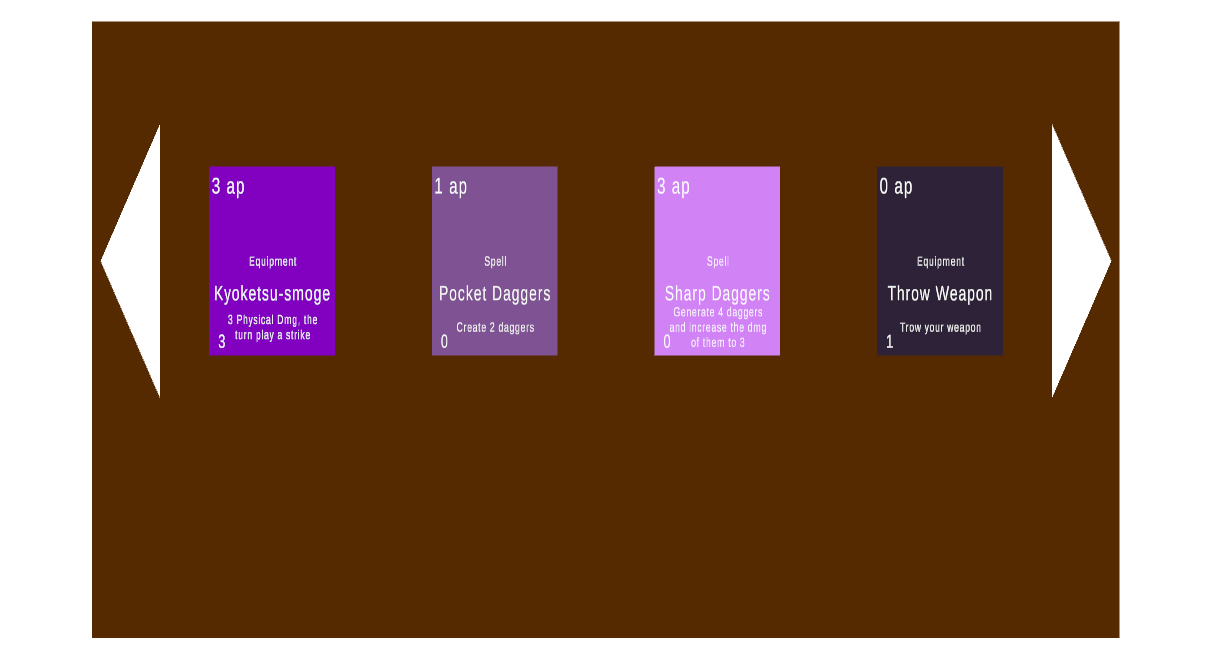
\includegraphics[width=400px,keepaspectratio]{images/chooseCard.png}
        \caption {A menü ahonnan a kártyát választjuk}
        \label{Choose}
    \hspace{1em}
\end{figure}

\begin{figure}[h]
        \centering
        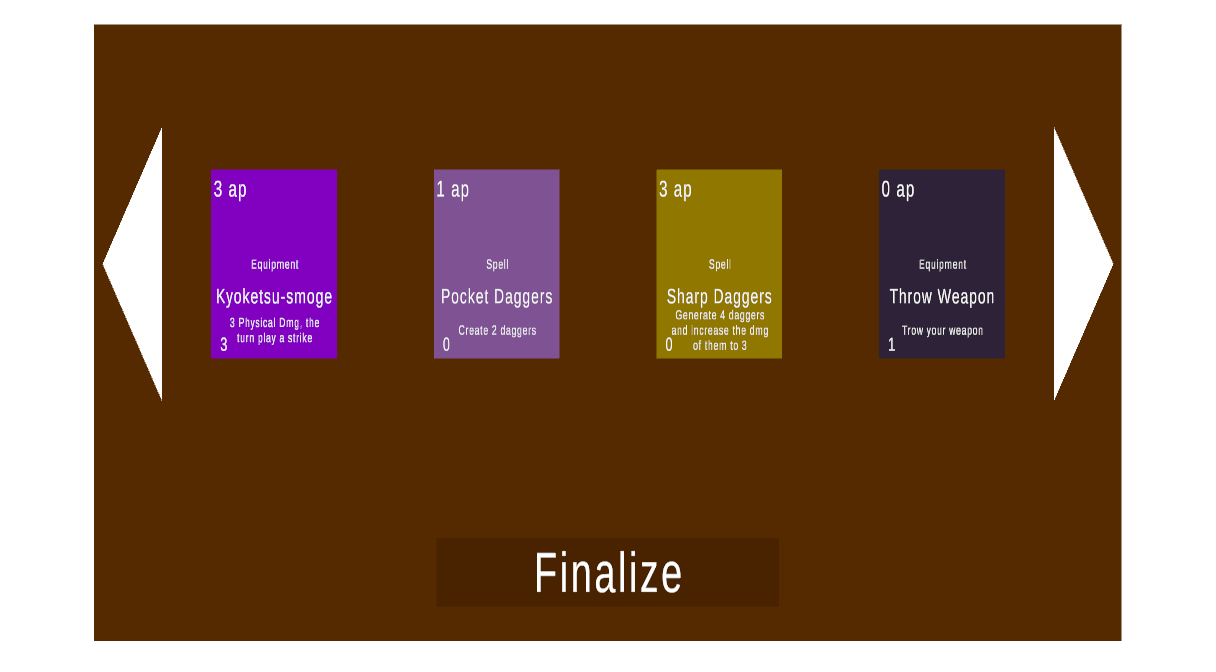
\includegraphics[width=400px,keepaspectratio]{images/cardChoosen.png}
        \caption {A menü kártya választás után}
        \label{Chosen}
    \hspace{1em}
\end{figure}
